\documentclass{article}
\usepackage[utf8]{inputenc}
\usepackage[margin=1.2in]{geometry}
\usepackage{hyperref}

\usepackage{listings}
\usepackage{xcolor}

\definecolor{codegreen}{rgb}{0,0.6,0}
\definecolor{codegray}{rgb}{0.5,0.5,0.5}
\definecolor{codepurple}{rgb}{0.58,0,0.82}
\definecolor{backcolour}{rgb}{0.95,0.95,0.92}

\lstdefinestyle{mystyle}{
    backgroundcolor=\color{backcolour},   
    commentstyle=\color{codegreen},
    keywordstyle=\color{magenta},
    numberstyle=\tiny\color{codegray},
    stringstyle=\color{codepurple},
    basicstyle=\ttfamily\footnotesize,
    breakatwhitespace=false,         
    breaklines=true,                 
    captionpos=b,                    
    keepspaces=true,                 
    numbers=left,                    
    numbersep=5pt,                  
    showspaces=false,                
    showstringspaces=false,
    showtabs=false,                  
    tabsize=2
}

\lstset{style=mystyle}


\usepackage{tikz}
\usetikzlibrary{positioning}

\usepackage{natbib}
\usepackage{graphicx}
\usepackage{amsmath}

\title{\vspace{-2 cm}Universidade Federal de Ouro Preto \\ PCC104 - Projeto e Análise de Algoritmos \\ Problemas $P$, $NP$ e $NP$-Completo}
\author{Prof. Rodrigo Silva}
%\date{}


\begin{document}

\maketitle

\section*{Instruções}

Cada aluno deve submeter na Plataforma Moodle um arquivo PDF com o nome no formato, \textit{seu\_nome\_semana3.pdf}, contendo:
\begin{itemize}
    \item Nome;
    \item Número de Matrícula; e
    \item Repostas das questões teóricas.
\end{itemize}

\section{Leitura Recomendada}

\begin{itemize}
    \item Seção 11.3 - \textit{Introduction to the Design and Analysis of Algorithms (3rd Edition)} - Anany Levitin 
\end{itemize}

\section{Atividades}

\begin{enumerate}
    \item O que significa dizer que um algoritmo resolve um problema em tempo polinomial?
    \item Que tipo de problemas considera-se tratável?
    \item Que tipo de problema considera-se intratável?
    \item Em ciência da computação, o que é o conjunto ou classe de problemas $P$?
    \item Como podemos provar que um problema pertence à classe $P$?
    \item O que é um problema decidível? E um problema indecidível?
    \item De forma geral, o que é um algoritmo determinístico?
    \item De forma geral, o que é um algoritmo não determinístico?
    \item Em ciência da computação, o que é o conjunto ou classe de problemas $NP$?
    \item O que é um algoritmo polinomial não determinístico?
    \item Explique por quê $P \subseteq NP$?
    \item Por quê saber se $P=NP$ é interessante?
    \item Como provamos que um problema é $NP$-Completo?
    \item Como provamos que um problema é $NP$-Completo quando já conhecemos algum problema $NP$-Completo?
    \item O que significaria resolver ao problema $NP$-Completo em $O(n^5)$?
    \item Um algoritmo que faz um número polinomial de chamadas a um procedimento que executa em tempo polinomial pode ter complexidade exponencial? Explique.
    \item Qual dos diagramas abaixo não contradiz o estado corrente do nosso conhecimento sobre as classes de problemas $P$, $NP$ e $NP$-Completo.
        \begin{figure}[!ht]
        \centering
        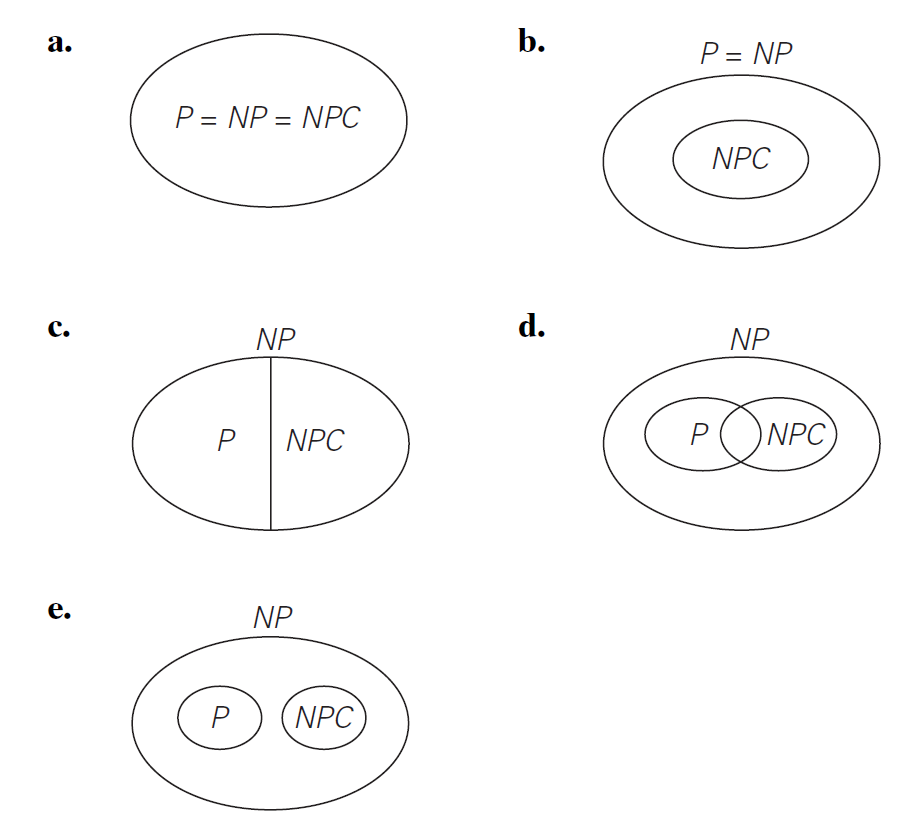
\includegraphics[width=0.7\textwidth]{Capture.PNG}
        \label{fig:my_label}
    \end{figure}
    \item Mostre que o Problema do Conjunto independente é um problema NP-Completo utilizando a redução entre problemas, considerando o 3-SAT como problema base.
    
\end{enumerate}



%\bibliographystyle{plain}
%\bibliography{references}
\end{document}

